% !TeX root = ../tfg.tex
% !TeX encoding = utf8

\chapter{Redes neuronales convolucionales}

Las \textbf{redes neuronales convolucionales} (CNNs) \cite{krizhevsky2012imagenet} son un tipo de modelo de ANN fundamental en el campo de la visión artificial y el procesamiento de imágenes. Fue introducido por Yann LeCun et al. en 1998 \cite{lecun1998gradient} y desde entonces ha sido ampliamente utilizado en una gran variedad de aplicaciones, desde problemas como la detección de objetos hasta la segmentación de imágenes.

\section{La corteza visual y el neocognitrón}

La comprensión del funcionamiento de la corteza visual en los seres humanos y otros animales ha sido una fuente de inspiración significativa para el desarrollo de algoritmos en el campo del aprendizaje profundo, especialmente en el diseño de CNNs. La corteza visual, ubicada en el lóbulo occipital del cerebro, es fundamental para el procesamiento de información visual. Estudios realizados por Hubel y Wiesel en la década de 1960 demostraron que ciertas neuronas en la corteza visual responden preferentemente a bordes específicos y orientaciones espaciales dentro de una región visual limitada \cite{hubel1962receptive}. Estas neuronas, conocidas como \textbf{células de orientación selectiva}, muestran una organización jerárquica que permite la percepción compleja a partir de la combinación de respuestas simples.

Inspirado en estas observaciones, Kunihiko Fukushima desarrolló el \textbf{neocognitrón} en 1980, una red neuronal que es considerada uno de los precursores de las modernas CNNs \cite{fukushima1980neocognitron}. El neocognitrón fue diseñado para reconocer patrones visuales complejos de manera robusta frente a traslaciones y otras pequeñas distorsiones de la imagen. Esta red consta de múltiples capas que alternan entre capas convolucionales, que detectan características locales y capas que agregan las respuestas de los detectores de características sobre áreas locales (\autoref{fig:neocognitron}). La estructura de esta red capta de manera efectiva la forma en que la corteza visual procesa la información visual, implementando una forma primitiva de invarianza a la traslación y la capacidad de extraer características jerárquicas.

\begin{figure}[h]
	\centering
	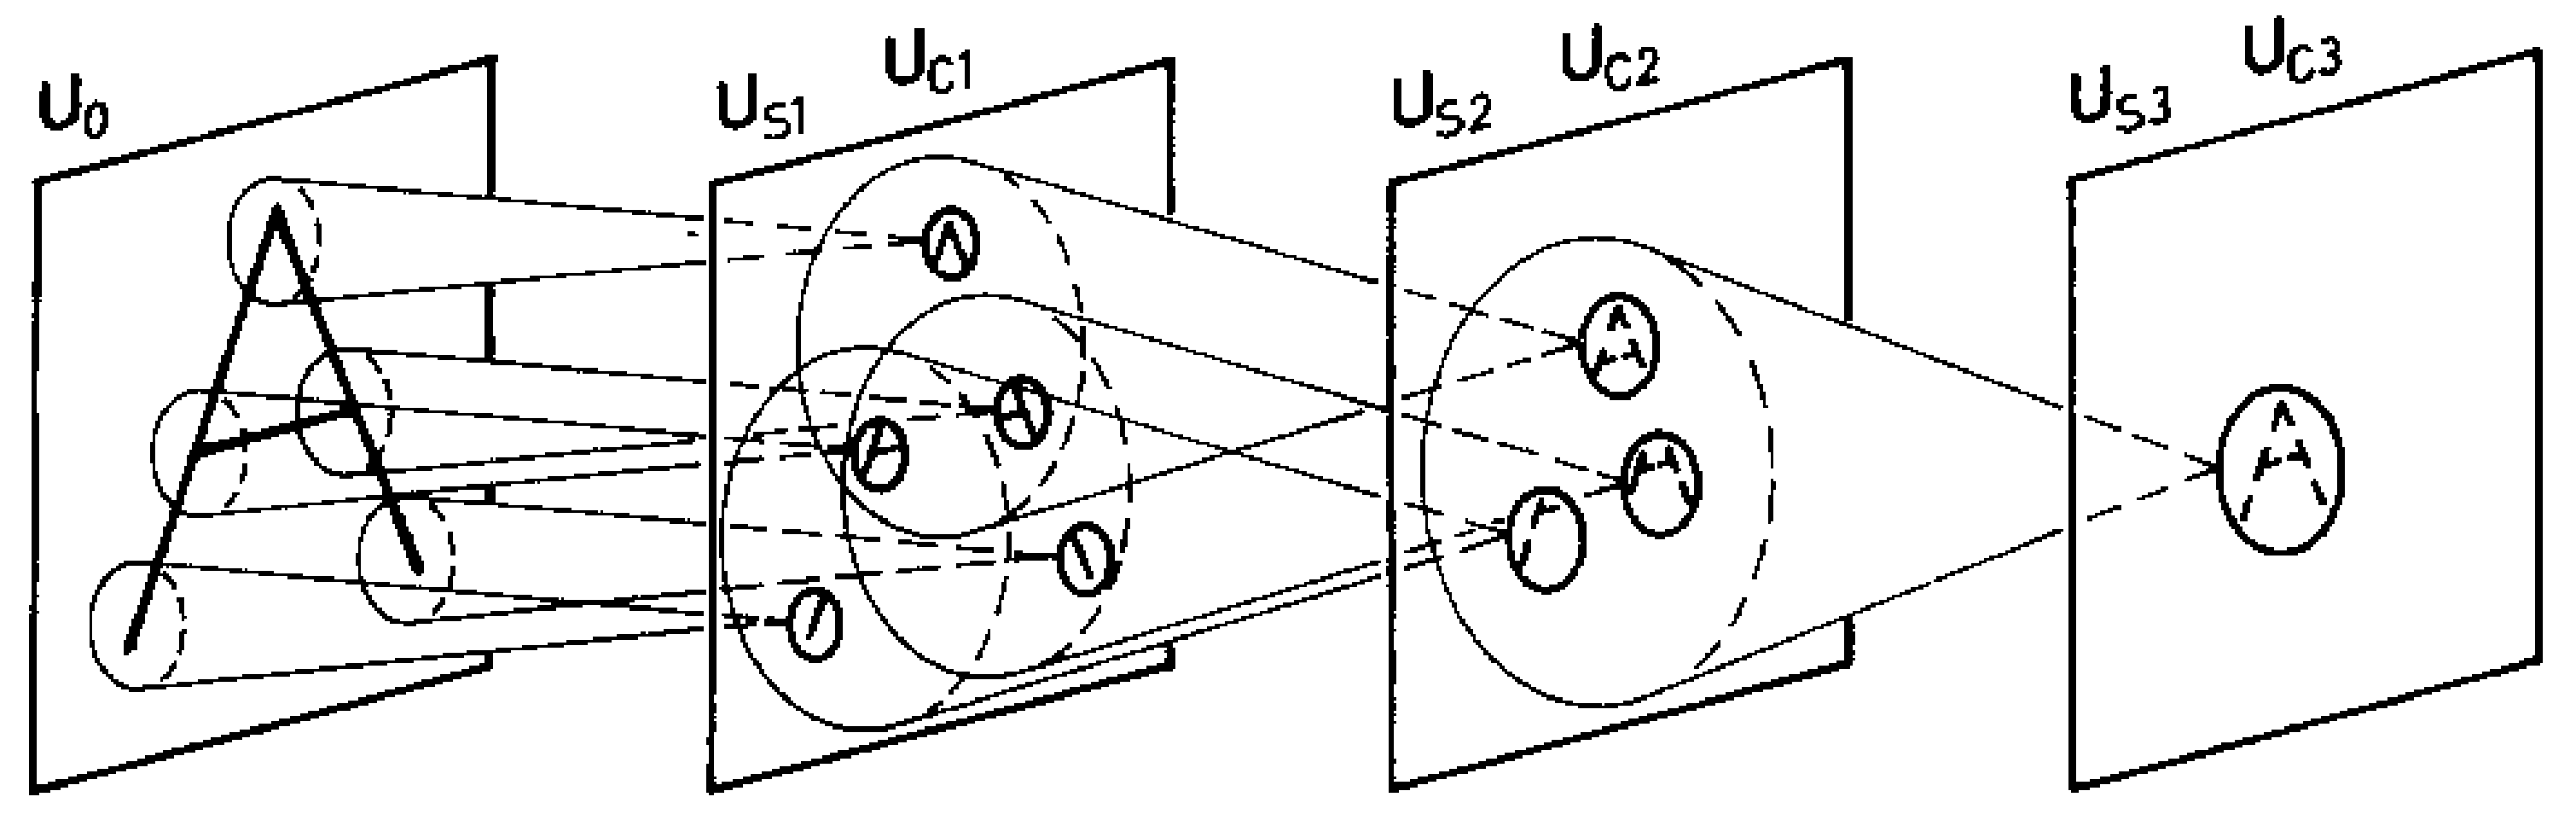
\includegraphics[width=110mm]{img/neocognitron.png}
	\caption{Diagrama del neocognitrón mostrando el flujo de procesamiento de una imagen a través de varias capas. Las capas \(U_{S}\) (simple) y \(U_{C}\) (compleja) procesan la información de forma jerárquica, comenzando con la imagen original \(U_0\) y extrayendo características cada vez más complejas en \(U_{S1}\), \(U_{C1}\), \(U_{S2}\), \(U_{C2}\), \(U_{S3}\) y \(U_{C3}\). Fuente \cite{fukushima1980neocognitron}.}
	\label{fig:neocognitron}
\end{figure}

La influencia de la corteza visual y el neocognitrón en el diseño de las CNNs es una muestra de la utilidad de estudios interdisciplinarios entre neurociencia y aprendizaje automático. Estos estudios no solo han facilitado avances tecnológicos en visión artificial sino que también han ofrecido nuevas perspectivas sobre cómo los seres humanos procesamos la información visual, proponiendo un puente entre la inteligencia artificial y la biológica \cite{serre2007feedforward}.


\section{Arquitectura de una CNN}

Las CNNs, introducidas por Yann LeCun, supusieron un avance significativo respecto al neocognitrón. Mientras que el neocognitrón sentó las bases al proponer una arquitectura inspirada en el procesamiento visual del cerebro, LeCun implementó un método de entrenamiento supervisado utilizando retropropagación, lo que permitió mejorar notablemente el rendimiento y la capacidad de generalización de las redes neuronales \cite{lecun1998gradient}. Además, LeCun sentó las bases de la arquitectura de CNNs, optimizando la eficiencia y escalabilidad de los modelos, incorporando capas como las capas convolucionales y de muestreo \cite{lecun1989backpropagation}.

\begin{figure}
% DEEP CONVOLUTIONAL NEURAL NETWORK
\centering
\begin{tikzpicture}[x=1.3cm,y=0.8cm]
	\large
	\message{^^JDeep convolution neural network}
	\readlist\Nnod{5,5,4,3,2,4,4,3} % array of number of nodes per layer
	\def\NC{6} % number of convolutional layers
	\def\nstyle{int(\lay<\Nnodlen?(\lay<\NC?min(2,\lay):3):4)} % map layer number on 1, 2, or 3
	\tikzset{ % node styles, numbered for easy mapping with \nstyle
		node 1/.style={node in},
		node 2/.style={node convol},
		node 3/.style={node hidden},
		node 4/.style={node out},
	}
	
	% TRAPEZIA
	\draw[myorange!40,fill=myorange,fill opacity=0.02,rounded corners=2]
	%(1.6,-2.5) rectangle (4.4,2.5);
	(1.6,-2.7) --++ (0,5.4) --++ (3.8,-1.9) --++ (0,-1.6) -- cycle;
	\draw[myblue!40,fill=myblue,fill opacity=0.02,rounded corners=2]
	(5.6,-2.0) rectangle++ (1.8,4.0);
	\node[font=\small,right=19,above=10,align=center,myorange!60!black] at (3.1,1.8) {Bloques\\[-0.2em]convolucionales};
	\node[font=\small,above=10,align=center,myblue!60!black] at (6.5,1.9) {Capas ocultas\\[-0.2em]totalmente conectadas};
	
	\message{^^J  Layer}
	\foreachitem \N \in \Nnod{ % loop over layers
		\def\lay{\Ncnt} % alias of index of current layer
		\pgfmathsetmacro\prev{int(\Ncnt-1)} % number of previous layer
		%\pgfmathsetmacro\Nprev{\Nnod[\prev]} % array of number of nodes in previous layer
		\message{\lay,}
		\foreach \i [evaluate={\y=\N/2-\i+0.5; \x=\lay; \n=\nstyle;}] in {1,...,\N}{ % loop over nodes
			%\message{^^J  Layer \lay, node \i}
			
			% NODES
			\node[node \n,outer sep=0.6] (N\lay-\i) at (\x,\y) {};
			
			% CONNECTIONS
			\ifnum\lay>1 % connect to previous layer
			\ifnum\lay<\NC % convolutional layers
			\foreach \j [evaluate={\jprev=int(\i-\j); \cconv=int(\Nnod[\prev]>\N); \ctwo=(\cconv&&\j>0);
				\c=int((\jprev<1||\jprev>\Nnod[\prev]||\ctwo)?0:1);}]
			in {-1,0,1}{
				\ifnum\c=1
				\ifnum\cconv=0
				\draw[connect,white,line width=1.2] (N\prev-\jprev) -- (N\lay-\i);
				\fi
				\draw[connect] (N\prev-\jprev) -- (N\lay-\i);
				\fi
			}
			
			\else % fully connected layers
			\foreach \j in {1,...,\Nnod[\prev]}{ % loop over nodes in previous layer
				\draw[connect,white,line width=1.2] (N\prev-\j) -- (N\lay-\i);
				\draw[connect] (N\prev-\j) -- (N\lay-\i);
			}
			\fi
			\fi % else: nothing to connect first layer
			
		}
	}
	
	% LABELS
	\node[font=\small,above=3,align=center,mygreen!60!black] at (N1-1.90) {Capa de\\[-0.2em]entrada};
	\node[font=\small, above=0,align=center,myred!60!black] at (N\Nnodlen-1.90) {Capa de\\[-0.2em]salida};
	
\end{tikzpicture}
\caption{Arquitectura de una CNN. Muestra la secuencia de capas en la red, iniciando con la capa de entrada, seguida por múltiples bloques convolucionales (resaltados en naranja), continuando con capas ocultas totalmente conectadas (resaltadas en azul) y finalmente la capa de salida. }
\end{figure}

Una CNN típicamente consiste en una secuencia de capas que transforman la entrada de imagen bruta en representaciones cada vez más abstractas y útiles para la tarea en cuestión. Cada tipo de capa dentro de una CNN tiene un propósito específico y contribuye de manera distinta al proceso de aprendizaje. Generalmente, las distintas capas de una CNN suelen agruparse para cumplir distintas funciones. Las principales agrupaciones que componen una CNN son:

\begin{itemize}
	\item \textbf{Capa de entrada}: Es la primera capa de la red, donde se introduce la imagen original o preprocesada. Su función principal es preparar y escalar la imagen para las operaciones de las capas siguientes.
	
	\item \textbf{Bloques convolucionales}: Estos bloques contienen una o más capas convolucionales seguidas frecuentemente por capas de normalización y funciones de activación. Cada capa convolucional aplica diferentes filtros a la entrada para crear mapas de características que resalten aspectos específicos de la imagen. Estos bloques suelen ir consecutivos intercalando capas de muestreo. 
	
	\item \textbf{Capas totalmente conectadas}: Después de varias capas convolucionales y de muestreo, la información en forma de matrices y tensores se aplana en vectores y se pasa a través de capas FC. Estas capas integran la información aprendida por las capas anteriores para realizar la clasificación final.
	
	\item \textbf{Capa de salida}: La última capa de una CNN, donde se obtiene el resultado final. En tareas de clasificación, esta capa suele usar una función de activación como la Softmax para asignar probabilidades a las distintas clases posibles.
\end{itemize}

A continuación, vamos a explorar las diferentes capas que componen estos bloques y cómo trabajan juntas para detectar y aprender patrones importantes en los datos.

\subsection{Capa convolucional}

La \textbf{capa convolucional} es el bloque de construcción fundamental de una CNN. Utiliza un conjunto de filtros que se aplican a la entrada mediante el operador de \textbf{convolución discreta}. Cada filtro detecta características específicas en una región local de la entrada. El operador de convolución discreta se puede expresar como:
\begin{equation}
	S(i, j) = (I \ast K)(i, j) = \sum_m \sum_n I(m, n) K(i-m, j-n),
\end{equation}
donde $m,n$ son las coordenadas en la imagen o matriz de entrada \(I\) de la región a convolucionar, $i,j$ son las coordenadas del centro del \textbf{kernel} o \textbf{filtro} \(K\) y \(S\) es la matriz de salida o \textbf{mapa de características}. La convolución discreta es un \textbf{operador lineal}, lo que implica que satisface propiedades como la \textbf{conmutatividad}, \textbf{asociatividad} y \textbf{distributividad}.

Estos filtros se desplazan sobre toda la superficie de la entrada, generando un mapa de características que resume la presencia de las particularidades de dicha entrada.

\usetikzlibrary{positioning, calc, decorations.pathreplacing}
\begin{figure}[H]
	\centering
\begin{tikzpicture}[
	2d-arr/.style={matrix of nodes, row sep=-\pgflinewidth, column sep=-\pgflinewidth, nodes={draw, text height=1.0ex, text depth=0.25ex}}
	]
	
	\matrix (mtr) [2d-arr] {
		0 & 1 & 1 & |[fill=orange!30]| 1 & |[fill=orange!30]| 0 & |[fill=orange!30]| 0 & 0\\
		0 & 0 & 1 & |[fill=orange!30]| 1 & |[fill=orange!30]| 1 & |[fill=orange!30]| 0 & 0\\
		0 & 0 & 0 & |[fill=orange!30]| 1 & |[fill=orange!30]| 1 & |[fill=orange!30]| 1 & 0\\
		0 & 0 & 0 & 1 & 1 & 0 & 0\\
		0 & 0 & 1 & 1 & 0 & 0 & 0\\
		0 & 1 & 1 & 0 & 0 & 0 & 0\\
		1 & 1 & 0 & 0 & 0 & 0 & 0\\
	};
	
	\node[below=of mtr-5-4] {$\mathbf I$};
	
	\node[right=0.2em of mtr] (str) {$*$};
	
	\matrix (K) [2d-arr, right=0.2em of str, nodes={draw, fill=teal!30}] {
		1 & 0 & 1 \\
		0 & 1 & 0 \\
		1 & 0 & 1 \\
	};
	\node[below=of K-3-2] {$\mathbf K$};
	
	\node[right=0.2em of K] (eq) {$=$};
	
	\matrix (ret) [2d-arr, right=0.2em of eq] {
		1 & 4 & 3 & |[fill=blue!80!black!30]| 4 & 1\\
		1 & 2 & 4 & 3 & 3\\
		1 & 2 & 3 & 4 & 1\\
		1 & 3 & 3 & 1 & 1\\
		3 & 3 & 1 & 1 & 0\\
	};
	\node[below=of ret-4-3] {$\mathbf{I * K}$};
	
	\draw[dashed, teal] (mtr-1-6.north east) -- (K-1-1.north west);
	\draw[dashed, teal] (mtr-3-6.south east) -- (K-3-1.south west);
	
	\draw[dashed, blue!80!black] (K-1-3.north east) -- (ret-1-4.north west);
	\draw[dashed, blue!80!black] (K-3-3.south east) -- (ret-1-4.south west);
	
	\foreach \i in {1,2,3} {
		\foreach \j in {4,5,6} {
			\node[font=\tiny, scale=0.6, shift={(-1.2ex,-2ex)}] at (mtr-\i-\j) {$\times \pgfmathparse{int(mod(\i+\j,2))}\pgfmathresult$};
		}
	}
	
\end{tikzpicture}
\caption{Ejemplo de convolución discreta. La matriz de entrada $\mathbf{I}$ se muestra con un segmento resaltado en naranja, mostrando la región afectada por el filtro $\mathbf{K}$, en color verde. La matriz resultante $\mathbf{I * K}$ destaca los valores resultantes de la convolución, con el resultado de la convolución en dicha región en azul.}
\end{figure}

Además de las propiedades del operador de convolución, las capas convolucionales muestran varias propiedades más que las hacen especialmente adecuadas para tareas de procesamiento de imágenes y visión artificial. Entre estas propiedades destacan:

\begin{itemize}
	\item \textbf{Conectividad local:}
	Cada neurona en una capa convolucional está conectada solo a un pequeño número de neuronas cercanas en la capa anterior. Esta estructura imita la manera en que los campos receptivos en el sistema visual humano se organizan, concentrándose en pequeñas regiones del espacio visual. La conectividad local permite a la red detectar características locales de la entrada sin la influencia de la estructura global, reduciendo la complejidad y el número total de parámetros necesarios.
	
	\item \textbf{Compartición de parámetros:}
	En una CNN, el mismo filtro se utiliza para cada posición de la entrada, a diferencia de una FNN donde cada peso es único para cada conexión. Esta compartición de parámetros permite que la red sea más eficiente en términos de memoria y computación. Además, también implica que las características aprendidas por un filtro son útiles en toda la imagen, lo que mejora la eficiencia del aprendizaje y ayuda a la red a generalizar mejor.
	
	\item \textbf{Equivarianza frente a traslaciones:}
	Debido al uso de la misma función de convolución a lo largo de toda la entrada, las CNNs son naturalmente equivariantes a las traslaciones. Esto significa que si la entrada se traslada, las características detectadas por la red también se trasladarán de manera correspondiente. Esta propiedad es particularmente interesante en tareas de visión artificial, donde la relevancia de una característica no suele depender de su posición específica en el espacio de entrada.
\end{itemize}

Los hiperparámetros de \textbf{paso} o \textbf{\textit{stride}}, y \textbf{relleno} o \textbf{\textit{padding}} son especialmente relevantes en la manipulación dimensional durante la convolución en CNNs. El \textit{stride} define el paso con el que el filtro se desplaza sobre la imagen o mapa de características, afectando la reducción dimensional del mapa resultante y permitiendo la captura de características a diversas escalas. Por otro lado, el \textit{padding} consiste en añadir píxeles artificiales alrededor de la imagen de entrada, lo que permite que el filtro acceda completamente a los bordes y mantiene el tamaño del volumen de salida, preservando la información en los bordes cruciales para la interpretación completa de la imagen.

\begin{figure}[H]
	\centering
	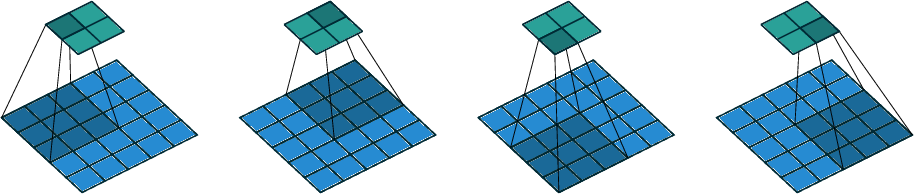
\includegraphics[width=100mm]{img/stride.png}
	\caption{Convolución de un filtro de 3x3 sobre una entrada de 5x5. La operación se realiza utilizando \textit{strides} de 2x2 y sin agregar relleno (\textit{padding} = 0), lo que resulta en una matriz de salida más pequeña y eficientemente espaciada. Fuente \cite{Dumoulin2016AGT}.}
\end{figure}
\begin{figure}[H]
	\centering
	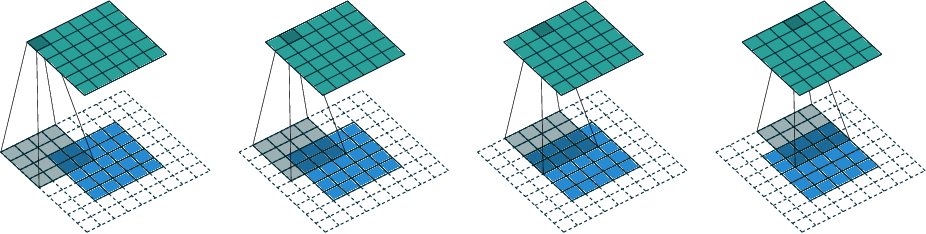
\includegraphics[width=100mm]{img/padding.png}
	\caption{Convolución de un filtro de 3x3 sobre una entrada de 5x5. Se emplea un relleno de 2 unidades y pasos unitarios (\textit{stride} = 1), asegurando que la matriz de salida aumente las dimensiones de la matriz de entrada, al expandir el borde de la imagen original. Fuente \cite{Dumoulin2016AGT}.}
\end{figure}

La elección de dichos hiperparámetros influye directamente en las dimensiones del mapa de características de salida, cuya altura \(H_{\text{out}}\) y anchura \(W_{\text{out}}\) vienen dadas de la siguiente manera:
\[
H_{\text{out}} = \left\lfloor \frac{H_{\text{in}} + 2P - H_{\text{f}}}{S} + 1 \right\rfloor, \quad
W_{\text{out}} = \left\lfloor \frac{W_{\text{in}} + 2P - W_{\text{f}}}{S} + 1 \right\rfloor,
\]
donde \(H_{\text{in}}\) y \(W_{\text{in}}\) son las dimensiones de entrada, \(H_{\text{f}}\) y \(W_{\text{f}}\) son las del filtro, \(P\) es el \textit{padding}, \(S\) es el \textit{stride} y $\lfloor \cdot \rfloor$ denota la función suelo. La profundidad del mapa de salida, \(D_{\text{out}}\), está determinada por el número de filtros aplicados, donde \( D_{\text{out}} = \text{número de filtros} \).

Estas convoluciones, aunque predominantemente asociadas con dimensiones bidimensionales, pueden extenderse a contextos tridimensionales (3D) donde se aplican filtros 3D sobre varios canales al mismo tiempo. Por ejemplo, un filtro de tamaño $1 \times 1 \times 1$ puede transformar linealmente los mapas de características en cada ubicación del volumen de entrada. Las dimensiones de salida se mantienen como:
\[
H_{\text{out}} = H_{\text{in}}, \quad W_{\text{out}} = W_{\text{in}}, \quad D_{\text{out}} = \text{número de filtros}.
\]
Nótese que estas convoluciones son importantes para ajustar la dimensionalidad de los canales dentro de redes profundas, pues con una sola \textbf{convolución $1 \times 1$} podemos colapsar todos los canales de entrada en uno solo. Esto supone una reducción efectiva de parámetros y de la complejidad computacional en datos tridimensionales.

Otro tipo de convoluciones que surge en este contexto son las \textbf{convoluciones en profundidad} o \textbf{\textit{depthwise convolutions}}. En ellas, cada filtro se aplica de manera independiente a cada canal del volumen de entrada, permitiendo un procesamiento separado de las dimensiones espaciales y de profundidad. La fórmula para las dimensiones de salida se mantiene, pero esta vez manteniendo el número de canales:
\[
H_{\text{out}} = \left\lfloor \frac{H_{\text{in}} + 2P - H_{\text{f}}}{S} + 1 \right\rfloor, \quad W_{\text{out}} = \left\lfloor \frac{W_{\text{in}} + 2P - W_{\text{f}}}{S} + 1 \right\rfloor, \quad D_{\text{out}} = D_{\text{in}}.
\]
Estas convoluciones son eficaces para optimizar el rendimiento computacional en aplicaciones donde el manejo eficiente de los recursos es esencial.

\subsection{Capa de muestreo}

Las capas de \textbf{muestreo}, conocidas generalmente como capas de \textbf{\textit{pooling}}, buscan reducir la dimensionalidad espacial de los mapas de características, lo que permite disminuir la cantidad de parámetros y de cómputo en la red al mismo tiempo que se mantiene la información más relevante. Las capas de \textit{pooling} más comunes son las de \textbf{máximo} o \textbf{\textit{max pooling}}, y las de \textbf{promedio} o \textbf{\textit{average pooling}}. El \textit{max pooling} toma la mayor activación en la ventana del filtro como:
\begin{equation}
	P(i, j) = \max_{m, n \in W} I(i+m, j+n),
\end{equation}
donde \(W\) es la ventana del filtro de \textit{pooling}. Esta operación ayuda a hacer la representación obtenida invariante a pequeñas traslaciones y distorsiones. Por otro lado, el \textit{average pooling} calcula el promedio de las activaciones dentro de la ventana del filtro, proporcionando una representación que suaviza las características de entrada:
\begin{equation}
	P(i, j) = \frac{1}{|W|} \sum_{a, b \in W} I(i+a, j+b),
\end{equation}
donde \(|W|\) es el número de elementos en la ventana del filtro. Ambas técnicas de pooling tienen sus aplicaciones específicas dependiendo de la naturaleza del problema y de la arquitectura de la red. Mientras que el \textit{max pooling} es generalmente preferido para tareas relacionadas con la detección de características debido a su capacidad para preservar las activaciones más fuertes, el \textit{average pooling} puede ser más adecuado para tareas donde la uniformidad de las características es más importante \cite{krizhevsky2012imagenet}.

\newcommand{\matrixA}{%     
	\setlength{\tabcolsep}{0pt}
	\begin{NiceTabular}{*{4}{c}}[hvlines,rules/width=2pt, cell-space-limits=1.0ex,columns-width=4ex]
		\CodeBefore % color the blocks
		\rectanglecolor{blue!15}{1-1}{2-2}
		\rectanglecolor{green!15}{3-1}{4-2}
		\rectanglecolor{orange!25}{1-3}{2-4}
		\rectanglecolor{red!15}{3-3}{4-4}
		\Body   
		\RowStyle[nb-rows=4]{\bfseries} % make all bold
		8&7&5&3\\
		12&9&5&7\\
		13&2&10&3\\
		9&4&5&14\\      
	\end{NiceTabular}
}

\newcommand{\matrixB}{% 
	\setlength{\tabcolsep}{0pt}
	\begin{NiceTabular}{*{2}{c}}[hvlines,rules/width=1.6pt,cell-space-limits=1.0ex,columns-width=4ex]
		\CodeBefore % color the cells
		\cellcolor{blue!15}{1-1}
		\cellcolor{orange!15}{1-2}
		\cellcolor{green!15}{2-1}
		\cellcolor{red!15}{2-2}
		\Body   
		\RowStyle[nb-rows=2]{\bfseries} % make all bold
		12&7\\
		13&14\\     
	\end{NiceTabular}
}

\newcommand{\matrixC}{% 
	\setlength{\tabcolsep}{0pt}
	\begin{NiceTabular}{*{2}{c}}[hvlines,rules/width=1.6pt,cell-space-limits=1.0ex, columns-width=4ex]
		\CodeBefore % color the cells
		\cellcolor{blue!15}{1-1}
		\cellcolor{orange!15}{1-2}
		\cellcolor{green!15}{2-1}
		\cellcolor{red!15}{2-2}
		\Body   
		\RowStyle[nb-rows=2]{\bfseries} % make all bold
		9&5\\
		7&8\\       
	\end{NiceTabular}
}

\begin{figure}
	\centering
\begin{tikzpicture}
	% layout the matrices
	\node (matA) {\matrixA};
	\node[ above right = -30pt and 150pt of matA, scale=1.2, anchor = south west] (matB) {\matrixB};
	\node[ below right = -20pt and 150pt of matA, scale=1.2, anchor =north  west] (matC) {\matrixC};
	% a large parenthesis
	\node (paren) [right = 120pt of matA] {$\left(\rule{0pt}{100pt}\right.$};
	% the arrow
	\draw[-latex,ultra thick,  shorten >=3mm, shorten <=2mm,] (matA.east) -- (paren.center)  node[midway,above, text width=3cm,     font= \bfseries, text centered] {2x2 pooling, stride 2};    
	% add the labels
	\node[above =  -3pt of matB.north,font=\bfseries]{Max pooling};
	\node[above =  -3pt of matC.north,font=\bfseries]{Average pooling};
\end{tikzpicture}  
\caption{Comparación de técnicas de \textit{pooling}. Arriba, \textit{max pooling} y abajo, \textit{average pooling}, ambas con un filtro de 2x2 y \textit{stride} de 2, mostrando la transformación de la matriz original.}
\end{figure}

%La \textbf{normalización} es un paso crucial en muchas CNNs que ayuda a acelerar la convergencia del entrenamiento y reduce la sensibilidad a la inicialización de los parámetros de la red. La normalización por lotes es una técnica común que normaliza las salidas de la capa anterior por mini-batch, ajustando y escalando las activaciones para tener una media cero y una varianza unitaria.
%
%\subsubsection{Capa totalmente conectada}
%
%Las capas FC en las CNNs desempeñan un papel importante al transformar las características extraídas por las capas convolucionales y de \textit{pooling} en predicciones finales. Al final de la arquitectura de la red, estas capas funcionan como clasificadores, interpretando las características y tomando decisiones basadas en ellas para clasificar la entrada en diferentes categorías. Además, en la \textbf{transferencia de aprendizaje} o \textbf{\textit{transfer learning}}, estas capas pueden ser reemplazadas o ajustadas para adaptarse a nuevas tareas, mientras que las capas convolucionales anteriores se utilizan para aprovechar las características genéricas aprendidas.

\section{Modelos y estado del arte en CNNs}

Desde su origen, las arquitecturas de CNNs han experimentado un desarrollo significativo, marcado por una serie de innovaciones que han mejorado su rendimiento y eficiencia. Como vimos anteriormente, la historia de las CNNs comenzó con el neocognitrón de Fukushima en los años 80 \cite{fukushima1980neocognitron}, un modelo novedoso que introdujo el concepto de capas convolucionales y de \textit{pooling}. Posteriormente, la introducción de LeNet-5 por LeCun et al. en los años 90 \cite{lecun1998gradient} demostró la eficacia de las CNNs en tareas de reconocimiento de dígitos y documentos, mostrando que este tipo de arquitecturas podían aprender a resolver problemas de aprendizaje supervisado. Posteriormente AlexNet, desarrollada por Krizhevsky et al. en 2012 \cite{krizhevsky2012imagenet}, revolucionó el campo del aprendizaje profundo, utilizando técnicas como paralización del entrenamiento, profundización de la red, ReLU y \textit{dropout} para ganar el desafío de ImageNet con una reducción drástica en la tasa de error. A partir de ahí, surgieron modelos más sofisticados como VGG \cite{simonyan2014very}, GoogLeNet con su módulo Inception \cite{szegedy2015going}, o ResNet, que introdujo las conexiones residuales permitiendo entrenar redes mucho más profundas \cite{he2016deep}. Cada una de estas arquitecturas ha contribuido a comprender mejor cómo diseñar redes eficientes para procesar y aprender de imágenes a gran escala. En la actualidad, modelos más recientes como DenseNet, que conecta cada capa directamente con todas las anteriores \cite{huang2017densely}, o EfficientNet, que escala de manera uniforme todas las dimensiones de la red \cite{tan2019efficientnet}, han logrado mejoras notables tanto en la eficiencia como en la capacidad de clasificación de las CNNs. Desde entonces, diferentes modelos de redes convolucioneales como EfficientNetV2 \cite{tan2021efficientnetv2smallermodelsfaster}, mejoras en el proceso de entrenamiento \cite{pham2021metapseudolabels} o el uso de novedosas arquitecturas como \textit{Transformer} \cite{NIPS2017_3f5ee243, dosovitskiy2021imageworth16x16words} continúan empujando los límites de lo que las CNNs pueden lograr, mejorando su capacidad de clasificación y optimizando su rendimiento y eficiencia para emplearlos en aplicaciones en tiempo real y en dispositivos con recursos limitados.

\subsection{ResNet}

Las \textbf{Redes Neuronales Residuales} (ResNet) introducidas por He et al. en 2015 \cite{he2016deep}, supusieron un avance significativo en la arquitectura de redes profundas para el reconocimiento de imágenes. A diferencia de sus predecesores como AlexNet y VGG, ResNet aborda el problema del desvanecimiento del gradiente que suele presentarse en redes muy profundas mediante la introducción de una conexión de identidad que salta una o más capas.

La clave de la arquitectura de ResNet es el \textbf{bloque residual}, que incorpora una \textbf{conexión residual} directamente conectando la entrada del bloque a su salida, lo que permite que la señal se propague directamente a través de la red. El bloque residual se puede expresar como:
\begin{equation}
	H(\mathbf{x}_l) = \mathcal{F}(\mathbf{x}_l, \{W_i\}) + \mathbf{x}_l
\end{equation}
donde \(\mathbf{x}_l\) y \(H(\mathbf{x}_l)\) son la entrada y la salida del $l$-ésimo bloque residual respectivamente, \(\mathcal{F}\) representa las capas intermedias de la red y \(\{W_i\}\) denota el conjunto de pesos de estas capas.

\begin{figure}
	\centering
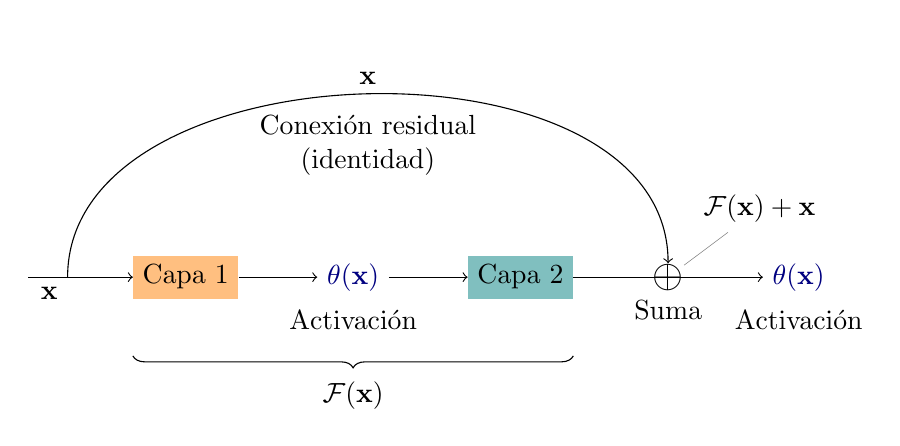
\begin{tikzpicture}
	
	\node[fill=orange!50] (l1) {Capa 1};
	\node[blue!50!black, right=of l1, label={below:Activación}] (act1) {$\theta(\mathbf{x})$};
	\node[fill=teal!50, right=of act1] (l2) {Capa 2};
	\node[right=of l2, font=\Large, label={below:Suma}, inner sep=0, pin={60:$\mathcal F(\mathbf{x}) + \mathbf{x}$}] (add) {$\oplus$};
	\node[blue!50!black, right=of add, label={below:Activación}] (act2) {$\theta(\mathbf{x})$};
	
	\draw[->] (l1) -- (act1);
	\draw[->] (act1) -- (l2);
	\draw[<-] (l1) -- ++(-2,0) node[below, pos=0.8] {$\mathbf{x}$};
	\draw[->] (l2) -- (act2) node[above, pos=0.8] {};
	\draw[->] ($(l1)-(1.5,0)$) to[out=90, in=90] node[below=1ex, midway, align=center] {Conexión residual\\(identidad)} node[above, midway] {$\mathbf{x}$} (add);
	\draw[decorate, decoration={brace, amplitude=1ex, raise=1cm}] (l2.east) -- node[midway, below=1.2cm] {$\mathcal F(\mathbf{x})$} (l1.west);
	
\end{tikzpicture}
\caption{Diagrama de una conexión residual. La entrada $\mathbf{x}$ pasa a través de la Capa 1 y una función de activación, fluyendo luego hacia la Capa 2. Paralelamente, $\mathbf{x}$ se suma directamente al final de la Capa 2 mediante una conexión residual. }
\end{figure}

A diferencia de AlexNet, que tiene 8 capas, y VGG, que tiene 16 o 19 capas, ResNet se diseñó con capacidades mucho más profundas, con versiones que van desde 18 hasta 152 capas. Lo revolucionario de ResNet no es simplemente añadir más capas, sino su habilidad para entrenar redes muy profundas sin sufrir desvanecimiento del gradiente gracias a sus conexiones residuales. Estas conexiones ayudan a preservar el gradiente a lo largo del proceso de aprendizaje, lo que permite entrenar redes más profundas que las posibles anteriormente.

El diseño del bloque residual permite que ResNet no solo evite el problema del desvanecimiento del gradiente sino que también mejore la eficiencia del entrenamiento. Los experimentos demuestran que las redes con bloques residuales superan a las arquitecturas convencionales en grandes conjuntos de datos de imágenes como ImageNet.

\subsection{DenseNet}

Las \textbf{Redes Convolucionales Densamente Conectadas} (DenseNet) propuestas por Huang et al. en 2017 \cite{huang2017densely}, representan otra evolución significativa en el diseño de redes neuronales profundas. DenseNet mejora la idea de conexiones de salto de ResNet mediante la integración de cada capa directamente con todas las capas posteriores de una manera densamente conectada.

La principal innovación de DenseNet es su estructura de \textbf{conexiones densas}, donde cada capa recibe como entrada todas las salidas de las capas anteriores, concatenando estas salidas. Esto se formula como sigue:
\begin{equation}
	\mathbf{x}_l = H_{l}([\mathbf{x}_0, \mathbf{x}_1, \dots, \mathbf{x}_{l-1}])
\end{equation}
donde \(\mathbf{x}_l\) es la salida de la capa \(l\), \([ \cdot ]\) denota la operación de concatenación y \(H_l\) es una función que representa las operaciones dentro de la capa \(l\), normalmente compuesta por operaciones de \textit{Batch Normalization}, activación ReLU, y convolución.

\begin{figure}
	\label{key}
	\centering
	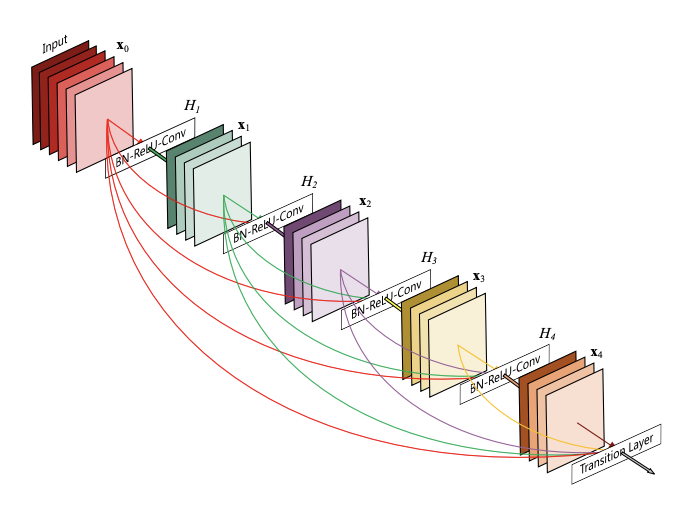
\includegraphics[width=100mm]{img/densenet.png}
	\caption{Arquitectura de DenseNet. La figura ilustra la configuración de la red DenseNet, mostrando cómo las capas están conectadas entre sí, donde cada capa recibe como entrada todas las salidas de las capas anteriores. Fuente \cite{huang2017densely}.}
\end{figure}

Aunque tanto ResNet como DenseNet utilizan conexiones que saltan capas, DenseNet ofrece una mejora en la eficiencia y la efectividad del entrenamiento al promover la reutilización de características de mayor manera. Mientras que las conexiones de salto en ResNet suman entradas, en DenseNet la información fluye a través de la red mediante la concatenación de características, lo que resulta en una mejora del flujo de información y gradientes a través de la red, reduciendo así el problema del desvanecimiento del gradiente de manera más efectiva.

DenseNet ha demostrado ser especialmente eficaz en conjuntos de datos como ImageNet y en aplicaciones donde la conservación de la información a lo largo de la red es crítica. Además, DenseNet tiende a ser más eficiente en términos de parámetros que ResNet debido a su capacidad para reutilizar características, lo que permite la construcción de redes profundas que son tanto compactas como potentes.

\subsection{EfficientNet}

\textbf{EfficientNet}, introducido por Tan y Le en 2019 \cite{tan2019efficientnet}, es un ejemplo de cómo se puede mejorar la eficiencia y la efectividad de las redes neuronales mediante una cuidadosa optimización de sus dimensiones. Lo innovador de EfficientNet es su metodología de escalado compuesto, que escala uniformemente todas las dimensiones de la red (profundidad, ancho y resolución de la imagen) con un conjunto fijo de coeficientes de escalado. La fórmula de escalado se representa como:

\begin{figure}
	\centering
	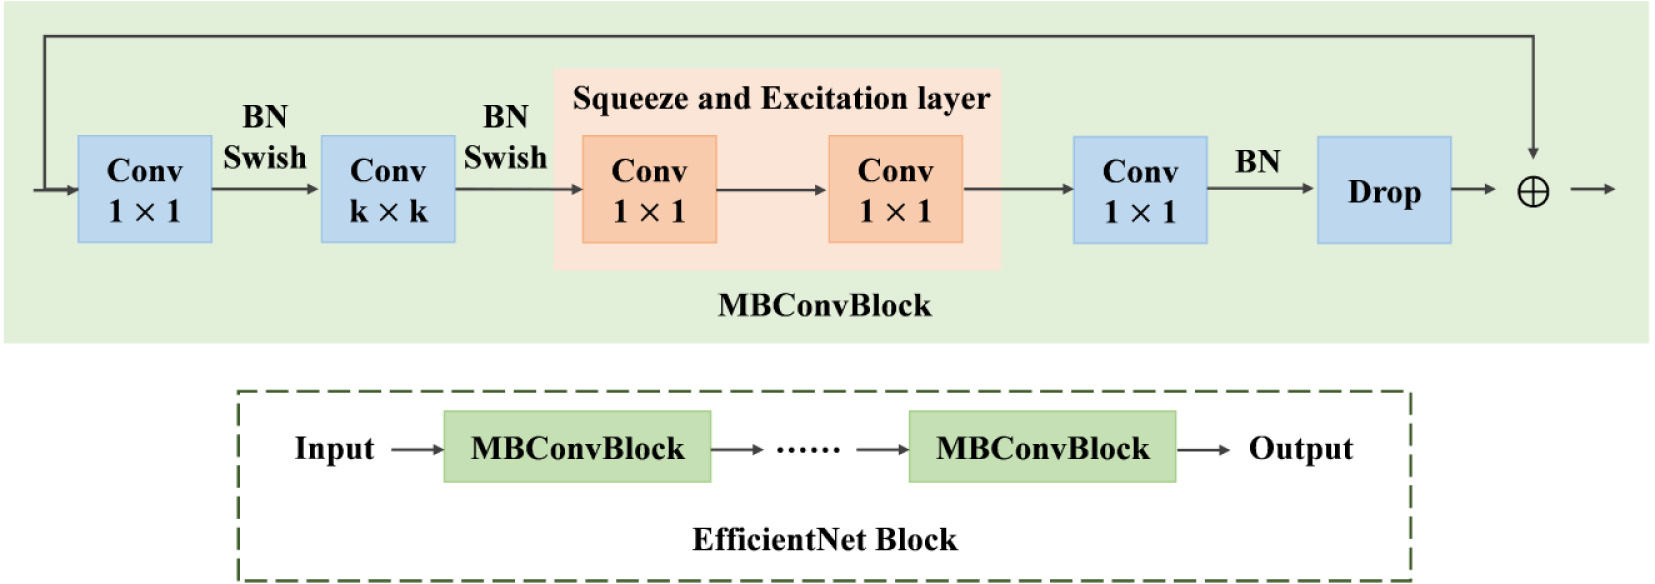
\includegraphics[width=140mm]{img/mbconv.jpg}
	\caption{Estructura de un bloque MBConv, la unidad básica en la arquitectura de EfficientNet.  Incluye capas convolucionales con activaciones Swish y normalización por lotes, intercaladas con capas SE para un refinamiento de las características. La secuencia de procesamiento termina en una capa de \textit{dropout} antes de la salida final. Fuente \cite{TANG2024105605}.}
\end{figure}

\begin{equation}
	\text{profundidad}: d = \alpha^\phi, \quad \text{anchura}: w = \beta^\phi, \quad \text{resolución}: r = \gamma^\phi,
\end{equation}
tal que 
\[
\alpha \cdot \beta^2 \cdot \gamma^2 \approx 2, \quad \alpha \geq 1, \quad \beta \geq 1, \quad \gamma \geq 1,
\]

donde \(\phi\) es un coeficiente que determina la cantidad de recursos disponibles para el escalado, y \(\alpha\), \(\beta\), \(\gamma\) son constantes que definen cómo deben escalar la profundidad, el ancho y la resolución, respectivamente, para lograr un equilibrio óptimo entre precisión y eficiencia.

\textbf{EfficientNet-B0} es el modelo base en la familia de modelos EfficientNet, que se caracteriza por aplicar un escalado uniforme a una arquitectura optimizada mediante \textbf{búsqueda de arquitectura neuronal} (NAS). La arquitectura inicia con una capa convolucional que maneja la imagen de entrada, aplicando la función de activación Swish y normalización por lotes para preparar las características para las etapas siguientes. A continuación, EfficientNet-B0 implementa una serie de \textbf{bloques MBConv}. Cada bloque MBConv sigue un patrón específico:

\begin{enumerate}
	\item \textbf{Expansión:} Primero, una convolución \(1 \times 1\) incrementa el número de canales. Esta técnica de expansión prepara los canales para una manipulación más intensiva, facilitando la extracción de características.
	
	\item \textbf{Convolución en profundidad:} A continuación, se aplica una convolución en profundidad con un filtro \(3 \times 3\) o \(5 \times 5\). Esta técnica permite la extracción de características locales de manera eficiente, sin un gran incremento en el número de parámetros como se observaría con convoluciones tradicionales.
	
	\item \textbf{Capa \textit{Squeeze and Excitation} (SE):} Esta capa sigue a la convolución en profundidad. Funciona primero reduciendo espacialmente cada canal a un valor escalar (\textit{squeeze}), que luego se utiliza para recalibrar los canales (\textit{excitation}) mediante operaciones de reescalado. Este proceso permite al modelo aprender a enfocar dinámicamente su atención en características informativas y suprimir las menos útiles.
	
	\item \textbf{Compresión:} Después de la capa SE, una convolución \(1 \times 1\) reduce el número de canales, consolidando las características importantes, lo cual asegura la eficiencia de la red y prepara la salida para la siguiente etapa del procesamiento.
\end{enumerate}

Las capas de reducción, situadas entre grupos de bloques MBConv, emplean convoluciones con un paso de 2 para reducir las dimensiones espaciales, aumentando el nivel de abstracción y reduciendo la carga computacional en las capas más profundas.

Finalmente, conexiones residuales se incorporan en cada bloque MBConv para facilitar el entrenamiento de la red al prevenir el desvanecimiento del gradiente. La red termina con una capa de muestreo promedio global que transforma la salida de los bloques MBConv en un vector único por imagen, el cual es procesado por una capa FC para realizar la clasificación final.

%A diferencia de ResNet y DenseNet, que principalmente se enfocan en mejorar la profundidad de la red o la densidad de las conexiones, EfficientNet proporciona un marco holístico que ajusta de manera equilibrada todas las dimensiones de la red. Esto no solo mejora el rendimiento sino que también aumenta la eficiencia del modelo, permitiendo que EfficientNet supere a modelos anteriores en precisión con un número significativamente menor de parámetros y una menor cantidad de operaciones de punto flotante (FLOPs).

\begin{figure}[hbt!]
	\centering
	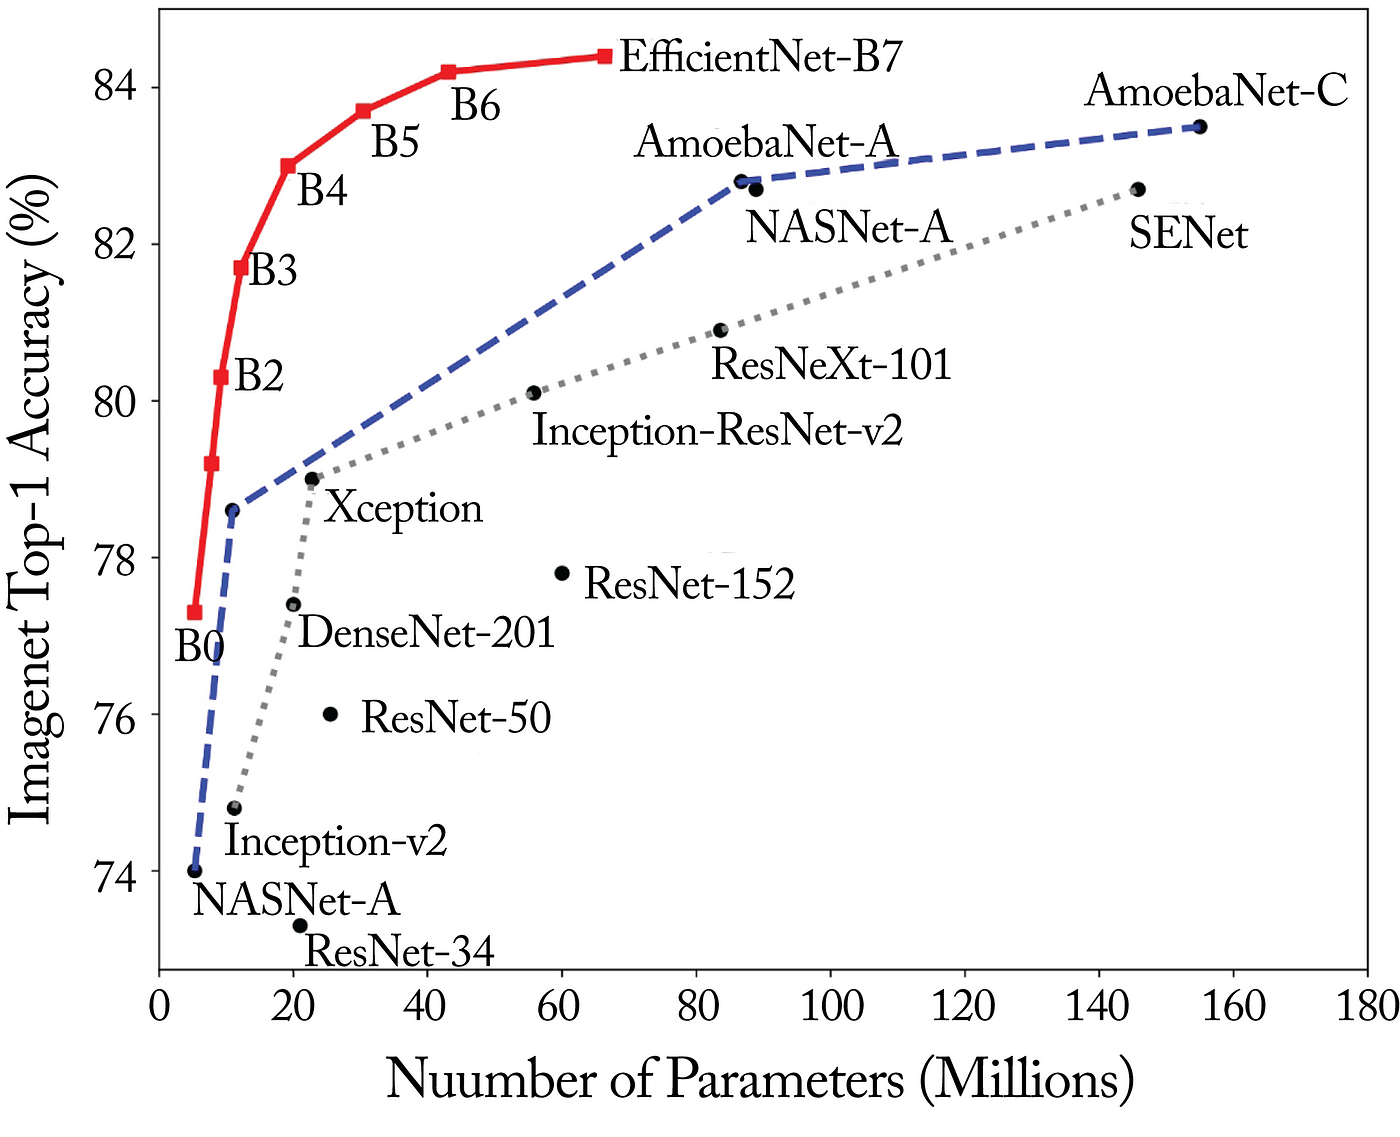
\includegraphics[width=100mm]{img/cnn-sota.png}
	\caption{Comparación de tamaño de modelo y precisión en ImageNet. EfficientNet supera notablemente al resto de modelos de CNNs. En general, EfficientNet muestra una mejora destacable en eficiencia y rendimiento comparado con modelos previos como ResNet-152. Fuente \cite{tan2019efficientnet}.}
\end{figure}

En la actualidad, modelos como ResNet, DenseNet y EfficientNet han establecido nuevos estándares de precisión en \textit{benchmarks} como \textbf{ImageNet}, donde las tasas de error se han reducido de manera significativa en comparación con los métodos tradicionales basados en características manuales. Estas arquitecturas avanzadas han demostrado no solo una gran capacidad de generalización sobre grandes conjuntos de datos, sino también robustez frente a variaciones y perturbaciones en las imágenes. Además, la integración de técnicas como el aumento de datos y la \textbf{transferencia de aprendizaje} o \textbf{\textit{transfer learning}}, han permitido aplicar modelos entrenados en un dominio específico a nuevos conjuntos de datos con poco o ningún ajuste adicional. Este progreso ha transformado la clasificación de imágenes de ser un desafío técnico a una herramienta útil, con aplicaciones en múltiples industrias, desde el reconocimiento automático de contenido en redes sociales hasta sistemas avanzados de asistencia al conductor en vehículos autónomos.

\endinput
%--------------------------------------------------------------------
% FIN DEL CAPÍTULO. 
%--------------------------------------------------------------------
